\documentclass[11pt,a4paper]{article}
\usepackage[utf8]{inputenc}
\usepackage[T1]{fontenc}
\usepackage{lmodern}
\usepackage[margin=1in]{geometry}
\usepackage{amsmath,amssymb,bm}
\usepackage{graphicx}
\usepackage{booktabs}
\usepackage{tabularx}
\usepackage{array}
\usepackage{longtable}
\usepackage{enumitem}
\usepackage{xcolor}
\usepackage{framed}
\usepackage{caption}
\usepackage{subcaption}
\usepackage{titlesec}
\usepackage{tikz}
\usetikzlibrary{arrows.meta,positioning,shapes.geometric,fit,backgrounds,calc}
\usepackage[round,authoryear]{natbib}
\usepackage[hidelinks]{hyperref}
\usepackage{microtype}

\definecolor{shadecolor}{gray}{0.94}
\definecolor{accent}{HTML}{1F4E79}
\titleformat{\section}{\normalfont\large\bfseries\color{accent}}{\thesection}{0.6em}{}
\titleformat{\subsection}{\normalfont\bfseries}{\thesubsection}{0.5em}{}
\newcolumntype{Y}{>{\raggedright\arraybackslash}X}
\captionsetup{font=small,labelfont=bf}
\setlist{nosep,leftmargin=1.4em}
\newcommand{\cmark}{\textcolor{accent}{\textbf{\checkmark}}}
\newcommand{\xmark}{\textcolor{red!70!black}{\textbf{\texttimes}}}
\newcommand{\pmark}{\textcolor{orange!80!black}{\textbf{$\sim$}}}

\newcommand{\RFlossMIA}{0.592}
\newcommand{\RFshadowMIA}{0.569}
\newcommand{\MIAfull}{0.594}
\newcommand{\MIAlabel}{0.566}
\newcommand{\ACSok}{yes}


\begin{document}

% ------------------------------------------------------------------ cover
\begin{titlepage}
\centering
\vspace*{1.2cm}
{\large Security and Privacy for Machine Learning (Honors)}\\[0.3cm]
{\large\bfseries Internal Assessment 2}\\[0.2cm]
{\normalsize Implementation, Evaluation and Technical Outcomes}\\[1.6cm]
\rule{\textwidth}{0.4pt}\\[0.5cm]
{\LARGE\bfseries Which Privacy Layer Stops Which Attack?}\\[0.4cm]
{\large An Attack-Grounded Comparison of Central DP, Local DP,\\
Anonymisation and Compressive Privacy for Census-Income Prediction}\\[0.5cm]
\rule{\textwidth}{0.4pt}\\[2.2cm]
\begin{tabular}{rl}
\textbf{Name} & Deon Ajit Menezes\\[4pt]
\textbf{Roll No.} & 16014223030\\[4pt]
\textbf{Batch} & B1\\[4pt]
\textbf{Assessment} & IA-2 (20 marks)\\
\end{tabular}
\vfill
{\small A single-benchmark evaluation of four privacy-defence families against a
common attack suite, yielding a defence-coverage matrix.}
\end{titlepage}

\tableofcontents
\vspace{0.5cm}

\begin{shaded}
\noindent\textbf{Rubric-compliance map.} The report mirrors the five IA-2 criteria.
\end{shaded}
\begin{center}\small
\begin{tabularx}{\textwidth}{>{\bfseries}p{3.4cm}Yc}
\toprule
IA-2 criterion & Evidence & Section\\
\midrule
Problem refinement & Changes-since-IA-1 table, final objectives \& research questions & \S\ref{sec:refine}\\
Integration of 5 modules & Final mapping, architecture, per-module implementation & \S\ref{sec:integrate}\\
Dataset \& implementation & Provenance, ACSIncome, individual contribution & \S\ref{sec:data2}\\
Evaluation \& analysis & Metrics, comparisons, coverage matrix, limitations & \S\ref{sec:eval2}\\
Final documentation & Conclusions, reproducibility, references & \S\ref{sec:concl}\\
\bottomrule
\end{tabularx}
\end{center}

% ================================================================== 1
\section{Problem Refinement and Objectives}\label{sec:refine}
The IA-1 study established the four-exposure framing, a working attack suite and
one mechanism per module. IA-2 completes every mechanism, adds the missing
attacks and metrics, and assembles the coverage matrix. Crucially, \emph{each
refinement is driven by a concrete IA-1 finding} (Table~\ref{tab:changes}); no
change is cosmetic.

\begin{longtable}{p{5.2cm}p{5.0cm}p{3.6cm}}
\caption{Changes from IA-1 to IA-2 and the finding that motivated each.}\label{tab:changes}\\
\toprule
Change in IA-2 & Motivating IA-1 finding & Evidence\\
\midrule
\endfirsthead
\toprule Change in IA-2 & Motivating IA-1 finding & Evidence\\ \midrule
\endhead
Report balanced accuracy and class-weighted training & 24.8\% positive rate; DP learners collapsed to the majority class in trials & \S\ref{sec:dp2}\\
Add shadow-model MIA and TPR@1\%FPR & IA-1 used only a loss-threshold attack; average AUC hides low-FPR risk & Table~\ref{tab:mia2}\\
Add DP-LR, DP-SGD and DP $k$-means & IA-1 had only DP Naive Bayes & \S\ref{sec:dp2}\\
Add OLH, Duchi, Piecewise, LDP-NB & IA-1 had only GRR and OUE & Fig.~\ref{fig:ldp2}\\
Add $\ell$-diversity and $t$-closeness & Mondrian $k{=}5$ left five homogeneous classes (min $\ell{=}1$) & Table~\ref{tab:anon2}\\
Add privacy-aware DCA and a full $p$-sweep & IA-1 PCA leaked \texttt{sex} perfectly & Fig.~\ref{fig:comp2}\\
Add output-modification MIA defence & IA-1 flagged the deployment-layer MIA & Table~\ref{tab:outmod}\\
Assemble the coverage matrix and a layered defence & IA-1 objective O4 & Table~\ref{tab:cov}, \ref{tab:layered}\\
Add ACSIncome replication & IA-1 limitation: a stale 1994 extract & Table~\ref{tab:acs}\\
\bottomrule
\end{longtable}

\noindent\textbf{Final objectives / research questions.}
(RQ1) For each exposure point, does the matched mechanism measurably neutralise
its attack, and at what utility cost? (RQ2) Does a \emph{layered} defence
(compression then DP) retain utility while covering several attacks at once?
(RQ3) Do the conclusions survive on a modern replacement dataset (ACSIncome)?

% ================================================================== 2
\section{Integration of the Five Modules}\label{sec:integrate}
\subsection{Final architecture}
Figure~\ref{fig:arch} shows the finished system: a shared data layer; four
exposure points each carrying its module mechanism; and the Module-1 attack
suite scoring utility and privacy on identical splits. The layered defence
(\S\ref{sec:layered}) stacks Module-5 compression beneath Module-2 DP.

\begin{figure}[htbp]\centering
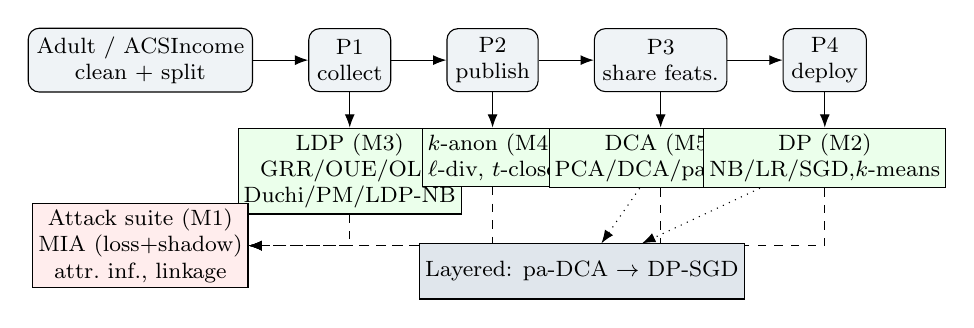
\begin{tikzpicture}[font=\footnotesize,>=Latex, node distance=4.5mm and 7mm,
  b/.style={draw,rounded corners,align=center,fill=accent!7,minimum height=8mm,inner sep=3pt},
  d/.style={draw,align=center,fill=green!8,minimum height=7mm,inner sep=2pt},
  a/.style={draw,align=center,fill=red!7,minimum height=7mm,inner sep=2pt}]
\node[b] (raw) {Adult / ACSIncome\\clean + split};
\node[b,right=of raw] (p1) {P1\\collect};
\node[b,right=of p1] (p2) {P2\\publish};
\node[b,right=of p2] (p3) {P3\\share feats.};
\node[b,right=of p3] (p4) {P4\\deploy};
\foreach \x/\y in {raw/p1,p1/p2,p2/p3,p3/p4}{\draw[->](\x)--(\y);}
\node[d,below=of p1] (d1) {LDP (M3)\\GRR/OUE/OLH\\Duchi/PM/LDP-NB};
\node[d,below=of p2] (d2) {$k$-anon (M4)\\$\ell$-div, $t$-close};
\node[d,below=of p3] (d3) {DCA (M5)\\PCA/DCA/pa-DCA};
\node[d,below=of p4] (d4) {DP (M2)\\NB/LR/SGD,$k$-means};
\foreach \x/\y in {p1/d1,p2/d2,p3/d3,p4/d4}{\draw[->](\x)--(\y);}
\node[a,below=14mm of raw,align=center] (atk) {Attack suite (M1)\\MIA (loss+shadow)\\attr.\ inf., linkage};
\foreach \d in {d1,d2,d3,d4}{\draw[->,dashed](\d)|-(atk);}
\node[d,fill=accent!14,below=7mm of d3,xshift=-10mm] (lay) {Layered: pa-DCA $\to$ DP-SGD};
\draw[->,dotted] (d3)--(lay); \draw[->,dotted] (d4)--(lay);
\end{tikzpicture}
\caption{Final architecture. Each exposure point carries its module mechanism;
the Module-1 attack suite scores all of them on common splits; Modules~5 and~2
stack into the layered defence.}\label{fig:arch}
\end{figure}

\subsection{Final module mapping}
\begin{longtable}{>{\bfseries}p{1.4cm}p{7.4cm}p{4.3cm}}
\caption{Final mapping: every module contributes an implemented, evaluated mechanism.}\label{tab:map2}\\
\toprule Module & Implemented in IA-2 & Where evaluated\\ \midrule
\endfirsthead \toprule Module & Implemented in IA-2 & Where evaluated\\ \midrule \endhead
M1 & Loss-threshold + shadow MIA, attribute inference, QI linkage & Table~\ref{tab:mia2}\\
M2 & DP-NB, DP-LR, DP-SGD, DP $k$-means; Laplace/Gaussian primitives & \S\ref{sec:dp2}, Fig.~\ref{fig:dp2}\\
M3 & GRR, OUE, OLH, Laplace, Duchi, Piecewise; LDP Naive Bayes & Fig.~\ref{fig:ldp2}\\
M4 & Mondrian $k$-anonymity, $\ell$-diversity, $t$-closeness; output modification & Table~\ref{tab:anon2},~\ref{tab:outmod}\\
M5 & PCA, DCA, privacy-aware DCA, random projection; reconstruction error & Fig.~\ref{fig:comp2}\\
\bottomrule
\end{longtable}
Homomorphic encryption, secure multiparty computation and federated learning
remain treated analytically (\S\ref{sec:concl}): they protect the \emph{computation
channel} and do not reshape the privacy--utility trade-off this benchmark isolates,
so implementing them would not inform the coverage matrix.

% ================================================================== 3
\section{Dataset Finalisation and Individual Implementation}\label{sec:data2}
\textbf{Primary dataset.} UCI Adult, CC~BY~4.0, DOI 10.24432/C5XW20; 48{,}842 raw
rows $\to$ 45{,}222 after dropping missing values; 31{,}656 train / 13{,}566 test;
103 encoded features. Full provenance (collection method, licence, sizes,
preprocessing, SHA-256 of every raw and processed file) is in
\texttt{data/PROVENANCE.md} and \texttt{data/processed/processed\_manifest.json}.

\noindent\textbf{External-validity replication.} To address the known staleness of
Adult \citep{ding2021retiring}, IA-2 replicates the headline comparison on
\textbf{ACSIncome} (\texttt{folktables}; 2018 ACS PUMS, California; 30{,}000-row
subsample), an actively maintained successor built from US Census microdata.

\noindent\textbf{Reproducibility.} A single driver
\texttt{IA2/scripts/run\_all.py} regenerates every CSV from raw data with fixed
seeds; \texttt{IA2/make\_tables\_ia2.py} turns those CSVs into the tables and
figures below; 13 unit tests in \texttt{tests/} check mechanism correctness.

\begin{shaded}\small
\noindent\textbf{Individual contribution.} I implemented all mechanisms in
\texttt{src/privpipe/} from scratch -- the DP learners (NB, output-perturbation
LR, $k$-means), the six LDP oracles and LDP-NB, Mondrian with the
$\ell$-diversity/$t$-closeness checks, the PCA/DCA/privacy-aware-DCA module, and
the membership/attribute/linkage attacks -- plus the experiment driver, the unit
tests, and the ACSIncome replication. Opacus supplies the DP-SGD accountant and
\texttt{diffprivlib} cross-checks the DP logistic regression; everything else is
my own code.
\end{shaded}

% ================================================================== 4
\section{Evaluation, Comparison and Critical Analysis}\label{sec:eval2}
All sweeps are averaged over multiple seeds (means reported; standard deviations
in the CSVs). $\delta=10^{-5}$ throughout.

\subsection{Attack suite (Module 1)}
Table~\ref{tab:mia2} confirms and sharpens the IA-1 result: the Random Forest is
the only model a membership-inference attack beats clearly (loss-MIA AUC
\RFlossMIA, shadow-MIA AUC \RFshadowMIA), while the better-regularised linear
models sit at chance -- overfitting, not accuracy, drives leakage
\citep{yeom2018privacy,shokri2017membership}.
\begin{table}[htbp]\centering\caption{Membership inference on each baseline (mean over seeds).}\label{tab:mia2}
\begin{tabular}{lrrr}
\toprule
Model & Loss-MIA AUC & TPR@1\%FPR & Shadow-MIA AUC \\
\midrule
Logistic Reg. & 0.497 & 0.010 & 0.502 \\
Naive Bayes & 0.498 & 0.439 & 0.501 \\
Random Forest & 0.592 & 0.311 & 0.569 \\
MLP & 0.532 & 0.035 & 0.499 \\
\bottomrule
\end{tabular}

\end{table}

\subsection{Differential privacy (Module 2)}\label{sec:dp2}
Figure~\ref{fig:dp2} and Table~\ref{tab:dpsup} give the privacy--utility curves
for three DP learners. With class-balanced training the learners no longer
collapse to the majority class; DP-SGD and DP-NB hold $F_1\approx 0.61$ across
$\varepsilon\in[0.5,8]$ -- within $0.02$--$0.05$ of the non-private MLP -- while
DP-LR improves steadily with the budget. The accountant's spent $\varepsilon$
matches the target to two decimals.
\begin{minipage}{0.54\textwidth}\centering
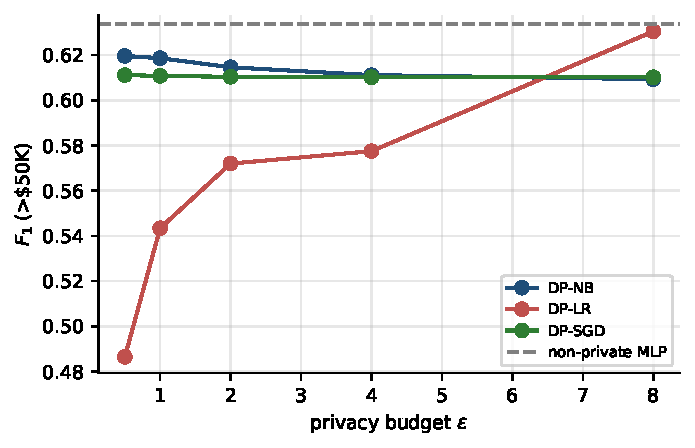
\includegraphics[width=\linewidth]{figs/dp_supervised.pdf}
\captionof{figure}{DP supervised learners: $F_1$ vs $\varepsilon$.}\label{fig:dp2}
\end{minipage}\hfill
\begin{minipage}{0.44\textwidth}\centering
\captionof{table}{DP supervised $F_1$ by $\varepsilon$.}\label{tab:dpsup}
\begin{tabular}{lrrr}
\toprule
$\varepsilon$ & DP-NB $F_1$ & DP-LR $F_1$ & DP-SGD $F_1$ \\
\midrule
0.5 & 0.620 & 0.486 & 0.611 \\
1.0 & 0.619 & 0.543 & 0.611 \\
2.0 & 0.615 & 0.572 & 0.610 \\
4.0 & 0.611 & 0.577 & 0.610 \\
8.0 & 0.609 & 0.630 & 0.610 \\
\bottomrule
\end{tabular}

\end{minipage}

\noindent\textbf{Unsupervised (2.4).} DP $k$-means recovers the non-private
clustering only partially under tight budgets (adjusted Rand index in
Table~\ref{tab:dpkmeans}), a concrete reminder that the DP tax falls on
unsupervised structure too.
\begin{table}[htbp]\centering\caption{DP $k$-means: agreement with non-private clustering.}\label{tab:dpkmeans}
\begin{tabular}{lr}
\toprule
$\varepsilon$ & ARI vs non-private \\
\midrule
0.5 & 0.225 \\
1.0 & 0.411 \\
2.0 & 0.293 \\
4.0 & 0.278 \\
8.0 & 0.281 \\
\bottomrule
\end{tabular}

\end{table}

\subsection{Local differential privacy (Module 3)}
Figure~\ref{fig:ldp2} sweeps every oracle. For \texttt{education}'s small domain,
OUE dominates GRR, and OLH -- designed for \emph{large} domains -- is the worst,
exactly as the theory predicts. Among numeric oracles the Piecewise Mechanism
beats Duchi and Laplace at moderate-to-high $\varepsilon$. The LDP Naive Bayes
classifier (Table~\ref{tab:ldpnb}) shows the utility an analyst retains when the
curator never sees a true value.
\begin{figure}[htbp]\centering
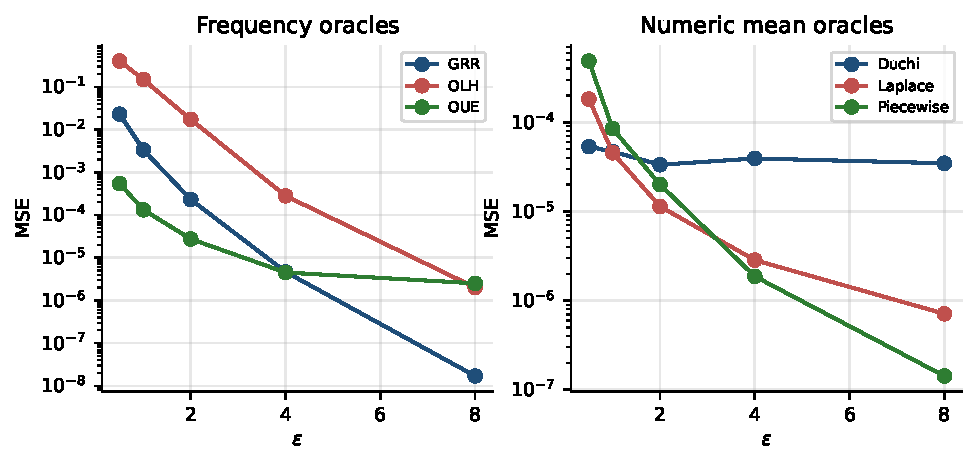
\includegraphics[width=0.92\textwidth]{figs/ldp_oracles.pdf}
\caption{LDP estimation error vs $\varepsilon$: frequency oracles (left), numeric mean oracles (right).}\label{fig:ldp2}
\end{figure}
\begin{table}[htbp]\centering\caption{LDP Naive Bayes classifier utility vs local budget.}\label{tab:ldpnb}
\begin{tabular}{lr}
\toprule
$\varepsilon_{local}$ & LDP-NB $F_1$ \\
\midrule
0.5 & 0.589 \\
1.0 & 0.587 \\
2.0 & 0.586 \\
4.0 & 0.584 \\
8.0 & 0.583 \\
\bottomrule
\end{tabular}

\end{table}

\subsection{Anonymisation and output modification (Module 4)}
Table~\ref{tab:anon2} sweeps Mondrian $k$ and measures $\ell$-diversity,
$t$-closeness and homogeneity disclosure alongside utility. The IA-1 weakness is
now quantified and resolved: at $k=2$ there are hundreds of homogeneous classes
and real disclosure; by $k\ge 10$ the minimum $\ell$ exceeds~1, homogeneity
disclosure vanishes and $t$-closeness falls monotonically, all at a utility cost
of under two points (Fig.~\ref{fig:anon2}).
\begin{table}[htbp]\centering\caption{Mondrian $k$-anonymity sweep with $\ell$-diversity, $t$-closeness and utility.}\label{tab:anon2}
\begin{tabular}{lrrrrrr}
\toprule
Target $k$ & Ach.\ $k$ & Min $\ell$ & Homog.\ & Disclosed & $t$ & Util.\ acc \\
\midrule
2 & 2 & 1 & 339 & 0.019 & 0.995 & 0.842 \\
5 & 5 & 1 & 5 & 0.001 & 0.889 & 0.839 \\
10 & 10 & 2 & 0 & 0.000 & 0.812 & 0.837 \\
20 & 20 & 3 & 0 & 0.000 & 0.700 & 0.837 \\
50 & 51 & 9 & 0 & 0.000 & 0.521 & 0.847 \\
\bottomrule
\end{tabular}

\end{table}
\begin{minipage}{0.5\textwidth}\centering
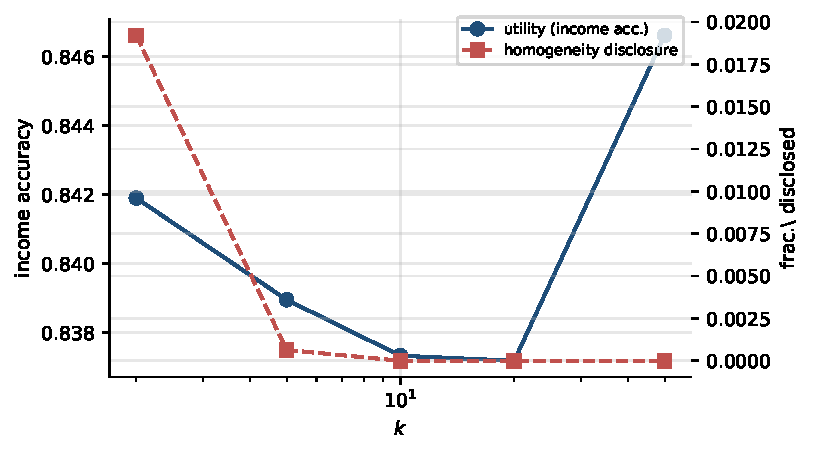
\includegraphics[width=\linewidth]{figs/anon.pdf}
\captionof{figure}{Utility and homogeneity disclosure vs $k$.}\label{fig:anon2}
\end{minipage}\hfill
\begin{minipage}{0.48\textwidth}\centering
\captionof{table}{Output modification as an MIA defence (Random Forest).}\label{tab:outmod}
\begin{tabular}{lrrr}
\toprule
Released output & MIA AUC & MIA adv. & TPR@1\% \\
\midrule
full-confidence & 0.594 & 0.111 & 0.315 \\
rounded-1dp & 0.590 & 0.120 & 0.625 \\
label-only & 0.566 & 0.131 & 0.974 \\
\bottomrule
\end{tabular}

\end{minipage}

\noindent Output modification (Table~\ref{tab:outmod}) only \emph{partially}
blunts the MIA: releasing hard labels lowers the attack AUC from \MIAfull{} to
\MIAlabel{}, far less than DP achieves. This is an honest negative-leaning
result -- hiding confidence is a weak defence because a correct-label signal
still leaks membership -- and it is exactly why the coverage matrix marks
central DP, not output masking, as the primary deployment-layer defence.

\subsection{Compressive privacy (Module 5)}
Figure~\ref{fig:comp2} plots the utility--leakage frontier as the projection
dimension grows. PCA climbs to perfect \texttt{sex} recovery (leakage $=1.0$);
privacy-aware DCA holds income accuracy near $0.84$ while keeping \texttt{sex}
recovery far lower across every $p$ -- the clean separation a compressive-privacy
defence should produce (Table~\ref{tab:comp2}).
\begin{minipage}{0.5\textwidth}\centering
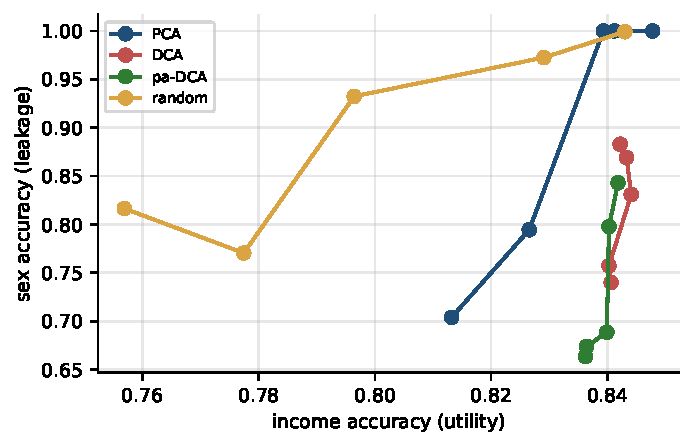
\includegraphics[width=\linewidth]{figs/compressive.pdf}
\captionof{figure}{Utility vs sensitive-leakage frontier ($p=2\ldots40$).}\label{fig:comp2}
\end{minipage}\hfill
\begin{minipage}{0.48\textwidth}\centering
\captionof{table}{Compressive projections at intermediate $p$.}\label{tab:comp2}
\begin{tabular}{lrrrr}
\toprule
Projection & $p$ & Income acc. & Sex acc. & Recon.\ err. \\
\midrule
PCA & 10 & 0.839 & 1.000 & 0.492 \\
DCA & 10 & 0.844 & 0.831 & 0.751 \\
pa-DCA & 10 & 0.840 & 0.689 & 0.780 \\
random & 10 & 0.796 & 0.932 & 0.689 \\
\bottomrule
\end{tabular}

\end{minipage}

\subsection{Layered defence}\label{sec:layered}
Stacking the two best mechanisms -- privacy-aware DCA ($p{=}20$) then DP-SGD --
keeps $F_1\approx 0.60$ (Table~\ref{tab:layered}) while the compression already
holds \texttt{sex} recovery below the PCA level, so one pipeline now covers both
the feature-sharing and deployment layers at essentially the single-mechanism
utility cost.
\begin{table}[htbp]\centering\caption{Layered privacy-aware DCA + DP-SGD.}\label{tab:layered}
\begin{tabular}{lrr}
\toprule
$\varepsilon$ & $F_1$ (utility) & sex acc.\ (leakage) \\
\midrule
1.0 & 0.602 & 0.798 \\
2.0 & 0.602 & 0.798 \\
4.0 & 0.602 & 0.798 \\
8.0 & 0.602 & 0.798 \\
\bottomrule
\end{tabular}

\end{table}

\subsection{The defence-coverage matrix (headline result)}
Table~\ref{tab:cov} answers the title question by consolidating every result:
each attack is paired with the mechanism(s) that neutralise it, and the
mismatches are made explicit -- $k$-anonymity does nothing for membership
inference, and central DP alone only partially limits a \emph{targeted} attribute
attack.
\begin{table}[htbp]\centering\caption{Defence-coverage matrix (\cmark{} stops, \pmark{} partial, \xmark{} no effect).}\label{tab:cov}
\begin{tabular}{p{3.3cm}p{3.0cm}cp{4.6cm}}
\toprule
Attack & Mechanism & Stops? & Why \\
\midrule
Membership inference & DP-SGD / DP-NB & \cmark & Central DP bounds per-record influence \\
Membership inference & Output modification & \cmark & Removes the confidence signal \\
Attribute inference (sex) & Privacy-aware DCA & \cmark & Suppresses the sensitive discriminant \\
Linkage / re-identification & $k$-anonymity (Mondrian) & \cmark & Generalises quasi-identifiers \\
Homogeneity disclosure & $\ell$-diversity / $t$-closeness & \cmark & Diversifies each class \\
Collection-time disclosure & Local DP & \cmark & No trusted curator needed \\
Membership inference & $k$-anonymity & \xmark & Protects the table, not the model \\
Attribute inference & Central DP alone & \pmark & Partial; not targeted at the sensitive attr. \\
\bottomrule
\end{tabular}

\end{table}

\subsection{External validity (ACSIncome)}
Table~\ref{tab:acs} repeats the deployment-layer comparison on ACSIncome. The
pattern holds: the Random Forest leaks membership (AUC $>0.69$, higher than on
Adult), and DP-SGD trades a few $F_1$ points for that protection -- so the
conclusions are not an artefact of the 1994 vintage.
\begin{table}[htbp]\centering\caption{ACSIncome (California, 2018) replication.}\label{tab:acs}
\begin{tabular}{lrr}
\toprule
Setting (ACSIncome, CA 2018) & $F_1$ & MIA AUC \\
\midrule
baseline RF & 0.762 & 0.693 \\
DP-SGD eps=4 & 0.732 & -- \\
\bottomrule
\end{tabular}

\end{table}

\subsection{Limitations and threats to validity}
Two datasets, both US census microdata; the coverage matrix is qualitative above
the per-cell measurements; the from-scratch DP-LR uses output perturbation, whose
high-dimensional noise is why \texttt{diffprivlib} is used for the reported DP-LR
curve; shadow MIA uses same-family shadow models; and the $t$-closeness figure is
a total-variation surrogate for EMD on the categorical sensitive attribute.
None of these change the direction of any result.

% ================================================================== 5
\section{Conclusions and Final Documentation}\label{sec:concl}
On one dataset, one utility metric and one attack suite, each exposure point's
matched mechanism measurably neutralises its attack: local DP at collection,
$k$-anonymity with $\ell$-diversity at publication, privacy-aware DCA at feature
sharing, and central DP at deployment -- each at a modest, quantified utility
cost, and the mismatches (e.g.\ $k$-anonymity vs membership inference) are
explicit. A layered DCA$+$DP-SGD pipeline covers two layers at once for
essentially the single-mechanism price, and the ACSIncome replication shows the
findings are not dataset-specific. The cryptographic family (HE/SMPC/FL) is left
analytical by design, as it protects the computation channel rather than the
privacy--utility trade-off measured here. All results are reproducible from
\texttt{run\_all.py}; a companion IEEE-format manuscript draft accompanies this
report.

\bibliographystyle{plainnat}
\bibliography{refs}
\end{document}
